\section{Estructura y organización del repositorio}

La implementación descrita en este manual se encuentra íntegramente versionada en un repositorio GitHub del proyecto, el cual contiene la totalidad del código fuente, playbooks, roles, inventarios, variables y plantillas necesarias para la configuración automatizada del clúster HPC. Este repositorio constituye la referencia operativa de la infraestructura como código desarrollada y permite reproducir el entorno mediante los procedimientos documentados en las secciones anteriores.

El repositorio puede consultarse en:

\begin{center}
\textbf{\href{https://github.com/JManuel-Mendoza/HPC-Ansible}{https://github.com/JManuel-Mendoza/HPC-Ansible}}
\end{center}

La descripción presentada en el presente capítulo se basa directamente en la estructura interna de dicho repositorio, de modo que cada componente conceptual expuesto previamente pueda asociarse con su ubicación concreta dentro del árbol de archivos. Esto permite identificar con precisión dónde se define cada servicio, variable o mecanismo de automatización.

\subsection{Vista general del proyecto}

La organización del repositorio materializa, en términos operativos, el modelo de automatización definido para el clúster: una base declarativa única, separación de responsabilidades y control explícito del estado. Por esa razón, en la raíz se concentran los puntos de entrada, el inventario y los directorios de configuración efectiva (\texttt{roles/}, \texttt{group\_vars/}, \texttt{host\_vars/}), mientras que los artefactos de soporte se mantienen fuera de la ruta de ejecución.

\begin{verbatim}
.
|-- site.yml
|-- cleanup_slurm_gpu.yml
|-- inventario.ini
|-- ansible.cfg
|-- requirements.yml
|-- group_vars/
|   |-- all/
|   `-- hpc_master.yml
|-- host_vars/
|   |-- master.yml
|   |-- worker1.yml
|   `-- worker2.yml
|-- roles/
|   |-- cluster_routing/
|   |-- common/
|   |-- firewall/
|   |-- llm_env/
|   |-- mariadb_server/
|   |-- munge/
|   |-- network_internal/
|   |-- nfs_hpc/
|   |-- nvidia_cuda/
|   |-- slurm_compute/
|   |-- slurm_controller/
|   |-- slurm_db_prep/
|   |-- slurm_facts/
|   |-- slurm_identities/
|   |-- slurm_install/
|   |-- slurm_rpm_build/
|   |-- slurm_validate/
|   |-- users_ssh/
|   `-- validate/
|-- docs/
|   |-- audit/
|   |-- docs_old/
|   `-- runbooks/
|-- tests/
`-- tools/
\end{verbatim}

Esta disposición prioriza trazabilidad: el lector puede identificar rápidamente qué archivos controlan el estado del clúster, cuáles ajustan comportamiento por grupo o nodo y cuáles cumplen función documental. El árbol orienta la ubicación física de los componentes, mientras la Tabla~\ref{tab:roles_mapa_operativo} resume su función operativa y alcance de ejecución.

\subsection{Playbook principal y puntos de entrada}

El punto de entrada canónico es \texttt{site.yml}. Su función estructural es actuar como contenedor principal de la definición declarativa del clúster, concentrando en un único archivo la referencia a los alcances de inventario y a los roles que componen la operación.

Junto a ese entrypoint existe \texttt{cleanup\_slurm\_gpu.yml}, destinado a escenarios de limpieza y reprovisión. La coexistencia de ambos playbooks responde a una separación intencional entre operación ordinaria y operación destructiva, evitando mezclar objetivos de naturaleza distinta en un mismo flujo.

\subsection{Organización de roles por dominios funcionales}

La carpeta \texttt{roles/} se estructura por dominios operativos del clúster y separa instalación, configuración y validación. Esta organización permite ubicar responsabilidades sin depender de la lectura completa de \texttt{site.yml}.

{\small
\begin{longtable}{|>{\raggedright\arraybackslash}p{2.4cm}|>{\raggedright\arraybackslash}p{3.1cm}|>{\raggedright\arraybackslash}p{3.5cm}|>{\raggedright\arraybackslash}p{5.1cm}|}
\caption{Mapa operativo de roles del repositorio\label{tab:roles_mapa_operativo}}\\
\hline
\textbf{Rol} & \textbf{Dominio funcional} & \textbf{Ejecuta principalmente en} & \textbf{Resultado principal} \\
\hline
\endfirsthead
\hline
\textbf{Rol} & \textbf{Dominio funcional} & \textbf{Ejecuta principalmente en} & \textbf{Resultado principal} \\
\hline
\endhead
\hline
\endfoot
\hline
\endlastfoot
\texttt{cluster\_routing} & Red\slash ruteo & \texttt{all} & Habilita forwarding y rutas entre segmentos internos para conectividad entre nodos del clúster. \\
\hline
\texttt{common} & Baseline & \texttt{all} & Instala paquetes base y servicios de sistema requeridos para operación homogénea. \\
\hline
\texttt{firewall} & Seguridad de red & \texttt{all} & Aplica reglas y puertos permitidos para SSH, Slurm y tráfico interno autorizado. \\
\hline
\texttt{llm\_env} & LLM\slash entorno & \texttt{all} & Prepara micromamba y dependencias Python para ejecución de cargas LLM. \\
\hline
\texttt{mariadb\_server} & Base de datos & \texttt{hpc\_master} & Instala y habilita MariaDB como backend de persistencia para contabilidad de Slurm. \\
\hline
\texttt{munge} & Seguridad Slurm & \texttt{slurm\_all} & Instala y configura Munge para autenticación entre componentes Slurm. \\
\hline
\texttt{network\_internal} & Red interna & \texttt{all} & Configura interfaces y direccionamiento de la red interna del clúster. \\
\hline
\texttt{nfs\_hpc} & Almacenamiento\slash NFS & \texttt{hpc\_master} y \texttt{all:!hpc\_master} & Configura export NFS en master y montajes cliente en nodos de cómputo. \\
\hline
\texttt{nvidia\_cuda} & GPU\slash CUDA & \texttt{all} (nodos con GPU) & Instala y ajusta stack NVIDIA/CUDA cuando el host reporta hardware acelerado. \\
\hline
\texttt{slurm\_compute} & Slurm\slash compute & \texttt{slurm\_compute} & Configura \texttt{slurmd} y parámetros de ejecución en nodos de cómputo. \\
\hline
\texttt{slurm\_controller} & Slurm\slash control & \texttt{hpc\_master} & Configura \texttt{slurmctld}/\texttt{slurmdbd} y activa servicios de control del scheduler. \\
\hline
\texttt{slurm\_db\_prep} & DB\slash Slurm accounting & \texttt{hpc\_master} & Crea base, usuarios y permisos requeridos por SlurmDBD en MariaDB. \\
\hline
\texttt{slurm\_facts} & Slurm\slash descubrimiento & \texttt{slurm\_all} & Recolecta hechos de CPU, memoria y GPU para parametrizar \texttt{slurm.conf} y GRES. \\
\hline
\texttt{slurm\_identities} & Identidades\slash Slurm & \texttt{slurm\_all} & Garantiza usuarios y grupos de servicio (\texttt{slurm}, \texttt{munge}) consistentes en todos los nodos Slurm. \\
\hline
\texttt{slurm\_install} & Slurm\slash instalación & \texttt{hpc\_master} y \texttt{slurm\_compute} & Instala paquetes Slurm y distribuye artefactos necesarios entre controlador y nodos compute. \\
\hline
\texttt{slurm\_rpm\_build} & Slurm\slash build & \texttt{hpc\_master} & Construye RPMs de Slurm en el nodo controlador para despliegue controlado. \\
\hline
\texttt{slurm\_validate} & Validación\slash Slurm & \texttt{hpc\_master} & Ejecuta pruebas de salud de Slurm y smoke tests sin modificar configuración. \\
\hline
\texttt{users\_ssh} & Acceso SSH & \texttt{all} & Endurece y valida configuración SSH para acceso administrativo al clúster. \\
\hline
\texttt{validate} & Validación general & \texttt{all} & Verifica estado de servicios y prerrequisitos operativos en todos los nodos. \\
\end{longtable}
}

\subsection{Jerarquía de variables}

En términos físicos, la configuración se reparte entre \texttt{roles/*/defaults/main.yml}, \texttt{group\_vars/} y \texttt{host\_vars/}. En la práctica del repositorio, \texttt{group\_vars/all/vars.yml} concentra parámetros transversales, \texttt{group\_vars/hpc\_master.yml} define ajustes del grupo controlador y \texttt{host\_vars/<hostname>.yml} encapsula particularidades de nodos concretos.

La precedencia aplicada sigue el patrón operativo del proyecto: primero defaults de rol, luego variables globales de \texttt{group\_vars/all}, después variables de grupo específico y, por último, overrides por host en \texttt{host\_vars/<hostname>.yml}. En caso de conflicto, prevalece el ámbito más específico, lo que hace explícito dónde se decide cada ajuste efectivo.

\subsection{Gestión de secretos}

Los secretos se ubican en \texttt{group\_vars/all/vault.yml}, archivo cifrado con Ansible Vault. Esta ubicación mantiene las credenciales fuera de los archivos de configuración en claro y preserva la separación entre parámetros públicos y material sensible.

La referencia a secretos se realiza mediante variables simbólicas \texttt{vault\_*} consumidas desde archivos no cifrados. Por ejemplo, \texttt{group\_vars/hpc\_master.yml} utiliza \texttt{vault\_slurmdb\_mysql\_password} para credenciales de base de datos, y el inventario define credenciales de elevación de grupo mediante claves \texttt{vault\_*}, sin exponer valores en texto plano.

\subsection{Documentación y artefactos auxiliares}

La carpeta \texttt{docs/} contiene documentación operativa y de gobernanza del repositorio: guías de referencia, runbooks, material de auditoría y notas de soporte. Su propósito es concentrar contexto de operación, criterios de validación y evidencia, sin mezclar esa información con la lógica ejecutable de los playbooks y roles.

En conjunto, esta distribución mantiene coherencia estructural entre código, variables, secretos y documentación, y conserva alineado el repositorio con el modelo de automatización adoptado. El resultado es un mapa técnico consistente que permite abordar el análisis del sistema con criterios sistemáticos, delimitando con precisión dónde reside cada decisión operativa.

\section{Servicio de red y conectividad interna}

\subsection{Propósito dentro del clúster}
La conectividad interna es la base operativa de todo el despliegue porque habilita, en cadena, la comunicación entre nodos, la publicación y montaje de NFS, el tráfico de control de Slurm y, finalmente, la ejecución distribuida de validaciones y cargas con GPU. En este repositorio, la red no se trata como una configuración manual por host, sino como un modelo declarativo gobernado por variables de inventario, de modo que el estado esperado de enlaces, direcciones y rutas queda descrito antes de ejecutar tareas.

Ese enfoque reduce ambigüedad en la operación: la topología se expresa en \path{group_vars/all/vars.yml}, y los roles de red la materializan sobre los nodos en función del inventario activo y de facts recolectados en cada play.

\begin{figure}[h]
\centering
{\shorthandoff{<>}
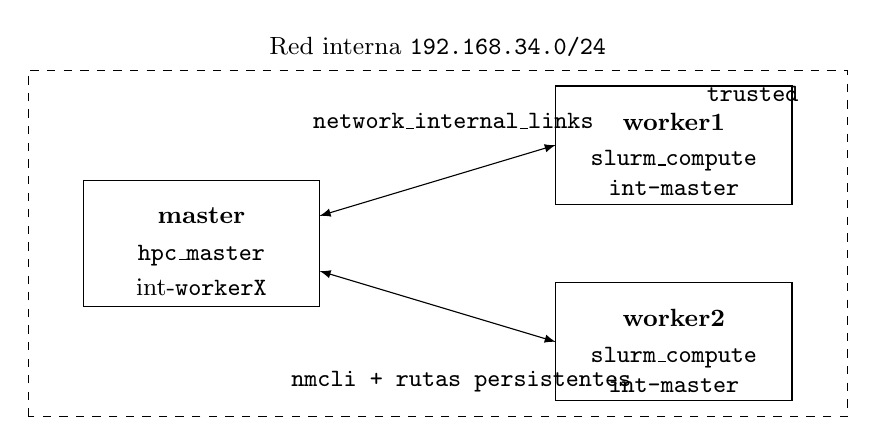
\begin{tikzpicture}[font=\small, >=latex]
  % Zona interna
  \draw[dashed] (-5.2,-2.2) rectangle (5.2,2.2);
  \node at (0,2.5) {Red interna \texttt{192.168.34.0/24}};
  \node at (4.0,1.9) {\texttt{trusted}};

  % Nodos
  \draw (-4.5,-0.8) rectangle (-1.5,0.8);
  \node at (-3.0,0.35) {\textbf{master}};
  \node at (-3.0,-0.15) {\texttt{hpc\_master}};
  \node at (-3.0,-0.55) {int-\texttt{workerX}};

  \draw (1.5,0.5) rectangle (4.5,2.0);
  \node at (3.0,1.55) {\textbf{worker1}};
  \node at (3.0,1.05) {\texttt{slurm\_compute}};
  \node at (3.0,0.7) {\texttt{int-master}};

  \draw (1.5,-2.0) rectangle (4.5,-0.5);
  \node at (3.0,-0.95) {\textbf{worker2}};
  \node at (3.0,-1.45) {\texttt{slurm\_compute}};
  \node at (3.0,-1.8) {\texttt{int-master}};

  % Enlaces bidireccionales
  \draw[<->] (-1.5,0.35) -- (1.5,1.25);
  \draw[<->] (-1.5,-0.35) -- (1.5,-1.25);

  % Etiquetas de interfaz/red
  \node at (0.2,1.55) {\texttt{network\_internal\_links}};
  \node at (0.3,-1.75) {\texttt{nmcli + rutas persistentes}};
\end{tikzpicture}
}
\end{figure}

\subsection{Modelo declarativo de topología}
La topología interna se define con \texttt{network\_internal\_links}, que mapea cada worker con su interfaz e IP en ambos extremos del enlace (\texttt{master\_if/master\_ip} y \texttt{worker\_if/worker\_ip}). Sobre esa base, \texttt{network\_internal\_keep\_if} protege la interfaz de gestión durante las operaciones de limpieza de conexiones, y las exclusiones (\texttt{network\_internal\_exclude\_ifaces} y \texttt{network\_internal\_exclude\_conn\_regex}) evitan tocar interfaces o conexiones no objetivo, como \texttt{tailscale0}.

El rol \texttt{network\_internal} impone este contrato al inicio; si la topología no está declarada, falla temprano para evitar una ejecución peligrosa en red.

\begin{filecode}{roles/network_internal/tasks/main.yml}
- name: Red Interna | Assert variables definidas
  ansible.builtin.assert:
    that:
      - network_internal_links is defined
      - network_internal_links is mapping
      - network_internal_links | length > 0
      - network_internal_keep_if is defined
      - network_internal_keep_if is string
      - network_internal_keep_if | length > 0
\end{filecode}

\subsection{Implementación sobre NetworkManager}
La implementación se realiza sobre NetworkManager mediante \texttt{nmcli}, invocado con \path{ansible.builtin.command} y, cuando hace falta filtrado en shell, con \path{ansible.builtin.shell}. El flujo operativo es introspectivo: primero lee conexiones existentes, decide qué conservar o eliminar según variables y estado actual, y luego crea o ajusta conexiones \texttt{int-*} para master y workers.

No se emplean plantillas estáticas de red para esta capa. En el repositorio no hay templates dedicados de red en estos roles, y la configuración depende del estado real del nodo (conexiones activas, interfaz detectada, pertenencia al inventario), por lo que la estrategia se basa en comandos idempotentes y verificación previa de valores actuales.

\subsection{Enrutamiento persistente}
El rol \texttt{cluster\_routing} completa la conectividad entre subredes internas. En el master habilita \texttt{net.ipv4.ip\_forward}; en workers calcula la subred local y deriva el gateway como la primera IP de esa subred (dirección de red + 1), usando la lista declarada en \texttt{hpc\_internal\_subnets}. Después añade rutas persistentes con \texttt{nmcli connection modify +ipv4.routes} y reactiva la conexión.

\begin{filecode}{roles/cluster_routing/tasks/main.yml}
- name: "WORKERS | Calcular subnet local, gateway (master) y rutas destino"
  ansible.builtin.command: python3 -
  args:
    stdin: |
      import ipaddress, os, json
      ip = ipaddress.ip_address(os.environ["NODE_IP"])
      subnets = [ipaddress.ip_network(s) for s in json.loads(os.environ["SUBNETS_JSON"])]
      ...
      gw = ipaddress.ip_address(int(local.network_address) + 1)
\end{filecode}

\subsection{Integración con firewall}
La integración con firewall se divide por responsabilidad de nodo. En el master, \texttt{cluster\_routing} mueve interfaces internas a zona \texttt{trusted}; en workers, confía la superred interna \texttt{192.168.34.0/24} como origen en esa misma zona. Encima de esa base, el rol \texttt{firewall} aplica reglas de servicio: abre SSH y añade \textit{rich rules} para tráfico Slurm desde \texttt{slurm\_internal\_cidr}, separando puertos y destino por rol de nodo (\texttt{6817/tcp} para \texttt{slurmctld} en master y \texttt{6818/tcp} para \texttt{slurmd} en workers).

Esta separación evita tratar el clúster como una superficie plana; cada regla queda asociada al tipo de host y al flujo esperado de control.

\subsection{Verificación operativa}
La verificación propia de red, dentro de la fase de red, se centra en estado operativo de conexiones NetworkManager: el rol consulta conexiones activas y reporta específicamente las internas \texttt{int-*}. También revisa rutas actuales en workers para comparar contra rutas deseadas antes de modificar persistencia.

No existe en el repositorio una validación dedicada de red con \texttt{ping} o asserts explícitos sobre \texttt{ip a}. La comprobación de conectividad termina de manera indirecta en validaciones de Slurm: \texttt{wait\_for} entre workers y controlador en \texttt{6817}, y desde master hacia workers en \texttt{6818}, además de chequeos de reglas \texttt{firewalld} esperadas.
